\documentclass[11pt,ignorenonframetext,]{beamer}
\setbeamertemplate{caption}[numbered]
\setbeamertemplate{caption label separator}{: }
\setbeamercolor{caption name}{fg=normal text.fg}
\beamertemplatenavigationsymbolsempty
\usepackage{lmodern}
\usepackage{amssymb,amsmath}
\usepackage{ifxetex,ifluatex}
\usepackage{fixltx2e} % provides \textsubscript
\ifnum 0\ifxetex 1\fi\ifluatex 1\fi=0 % if pdftex
  \usepackage[T1]{fontenc}
  \usepackage[utf8]{inputenc}
\else % if luatex or xelatex
  \ifxetex
    \usepackage{mathspec}
  \else
    \usepackage{fontspec}
  \fi
  \defaultfontfeatures{Ligatures=TeX,Scale=MatchLowercase}
\fi
\usetheme[]{metropolis}
% use upquote if available, for straight quotes in verbatim environments
\IfFileExists{upquote.sty}{\usepackage{upquote}}{}
% use microtype if available
\IfFileExists{microtype.sty}{%
\usepackage{microtype}
\UseMicrotypeSet[protrusion]{basicmath} % disable protrusion for tt fonts
}{}
\newif\ifbibliography
\hypersetup{
            pdftitle={Lecture 8},
            pdfauthor={Colin Rundel},
            pdfborder={0 0 0},
            breaklinks=true}
\urlstyle{same}  % don't use monospace font for urls
\usepackage{graphicx,grffile}
\makeatletter
\def\maxwidth{\ifdim\Gin@nat@width>\linewidth\linewidth\else\Gin@nat@width\fi}
\def\maxheight{\ifdim\Gin@nat@height>\textheight0.8\textheight\else\Gin@nat@height\fi}
\makeatother
% Scale images if necessary, so that they will not overflow the page
% margins by default, and it is still possible to overwrite the defaults
% using explicit options in \includegraphics[width, height, ...]{}
\setkeys{Gin}{width=\maxwidth,height=\maxheight,keepaspectratio}

% Prevent slide breaks in the middle of a paragraph:
\widowpenalties 1 10000
\raggedbottom

\AtBeginPart{
  \let\insertpartnumber\relax
  \let\partname\relax
  \frame{\partpage}
}
\AtBeginSection{
  \ifbibliography
  \else
    \let\insertsectionnumber\relax
    \let\sectionname\relax
    \frame{\sectionpage}
  \fi
}
\AtBeginSubsection{
  \let\insertsubsectionnumber\relax
  \let\subsectionname\relax
  \frame{\subsectionpage}
}

\setlength{\parindent}{0pt}
\setlength{\parskip}{6pt plus 2pt minus 1pt}
\setlength{\emergencystretch}{3em}  % prevent overfull lines
\providecommand{\tightlist}{%
  \setlength{\itemsep}{0pt}\setlength{\parskip}{0pt}}
\setcounter{secnumdepth}{0}

\usepackage{geometry}
\usepackage{graphicx}
\usepackage{amssymb}
\usepackage{color}          	% gives color options
\usepackage{url}		% produces hyperlinks
\usepackage[english]{babel}
\usepackage{colortbl}	% allows for color usage in tables
\usepackage{multirow}	% allows for rows that span multiple rows in tables
\usepackage{xcolor}		% this package has a variety of color options
\usepackage{calc}
\usepackage{multicol}
\usepackage{wrapfig}
\usepackage{textcomp}
\usepackage{bm}
\usepackage{bbm}
\usepackage{setspace}
\singlespacing

%%%%%%%%%%%%%%%%
% Small code output
%%%%%%%%%%%%%%%%

%% change fontsize of R code

%\let\oldShaded\Shaded
%\let\endoldShaded\endShaded
%\renewenvironment{Shaded}{\footnotesize\begin{spacing}{0.9}\oldShaded}{\endoldShaded\end{spacing}}

%% change fontsize of output
\let\oldverbatim\verbatim
\let\endoldverbatim\endverbatim
\renewenvironment{verbatim}{\footnotesize\begin{spacing}{0.9}\oldverbatim}{\endoldverbatim\end{spacing}}


\newcommand{\verbatimfont}[1]{\renewcommand{\verbatim@font}{\ttfamily#1}}

%%%%%%%%%%%%%%%%
% Custom Colors
%%%%%%%%%%%%%%%%

\xdefinecolor{oiBlue}{rgb}{0.15, 0.35, 0.55}
\xdefinecolor{gray}{rgb}{0.5, 0.5, 0.5}
\xdefinecolor{darkGray}{rgb}{0.3, 0.3, 0.3}
\xdefinecolor{darkerGray}{rgb}{0.2, 0.2, 0.2}
\xdefinecolor{rubineRed}{rgb}{0.89,0,0.30}
\xdefinecolor{linkCol}{rgb}{0.11,0.49,0.95}	
\xdefinecolor{irishGreen}{rgb}{0,0.60,0}	
\xdefinecolor{darkturquoise}{rgb}{0.44, 0.58, 0.86}
\definecolor{lightGreen}{rgb}{0.533,0.765,0.42}
%\xdefinecolor{hlblue}{rgb}{0.051,0.65,1}
\xdefinecolor{hlblue}{rgb}{ 0.055, 0.639, 0.831}
\definecolor{light}{rgb}{.337,.608,.741}
\definecolor{dark}{rgb}{.337,.608,.741}

\definecolor{cpink}{rgb}{0.93, 0.23, 0.51}

%%%%%%%%%%%%%%%%
% Custom Commands
%%%%%%%%%%%%%%%%

% text colors
\newcommand{\red}[1]{\textit{\textcolor{rubineRed}{#1}}}
\newcommand{\orange}[1]{\textit{\textcolor{orange}{#1}}}
\newcommand{\pink}[1]{\textit{\textcolor{rubineRed!90!white!50}{#1}}}
\newcommand{\green}[1]{\textit{\textcolor{irishGreen}{#1}}}
\newcommand{\blue}[1]{\textit{\textcolor{darkturquoise}{#1}}}
\newcommand{\light}[1]{\textcolor{light}{\textbf{#1}}}
\newcommand{\dark}[1]{\textcolor{dark}{#1}}
\newcommand{\gray}[1]{\textcolor{gray}{#1}}


% links: webURL, webLin, appLink
\newcommand{\webURL}[1]{\urlstyle{same}{\textit{\textcolor{linkCol}{\url{#1}}} }}
\newcommand{\webLink}[2]{\href{#1}{\textcolor{linkCol}{{#2}}}}
\newcommand{\appLink}[2]{\href{#1}{\textcolor{lightGreen!80!black!90}{{#2}}}}

% mail
\newcommand{\mail}[1]{\href{mailto:#1}{\textit{\textcolor{linkCol}{#1}}}}

% highlighting: hl, hlGr, mathhl
\newcommand{\hl}[1]{\textit{\textcolor{hlblue}{#1}}}
\newcommand{\hlGr}[1]{\textit{\textcolor{lightGreen}{#1}}}
\newcommand{\hlRd}[1]{\textit{\textcolor{rubineRed}{#1}}}
\newcommand{\mathhl}[1]{\textcolor{hlblue}{\ensuremath{#1}}}

% example
\newcommand{\ex}[1]{\textcolor{blue}{{{\small (#1)}}}}


\DeclareMathOperator*{\argmin}{arg\,min}
\DeclareMathOperator*{\argmax}{arg\,max}

\title{Lecture 8}
\subtitle{ARMA Models}
\author{Colin Rundel}
\date{02/13/2017}

\begin{document}
\frame{\titlepage}

\section{AR(p)}\label{arp}

\begin{frame}[t]{AR(p)}

From last time,

\[
\begin{aligned}
AR(p): \quad y_t 
  &= \delta + \phi_1 \, y_{t-1} + \phi_2 \, y_{t-2} + \cdots + \phi_p \, y_{t-p} + w_t  \\
  &= \delta + w_t + \sum_{i=1}^p \phi_i \, y_{t-i}
\end{aligned}
\]

What are the properities of \(AR(p)\),

\begin{enumerate}
\def\labelenumi{\arabic{enumi}.}
\item
  Expected value? \[~\]
\item
  Covariance / correlation? \[~\]
\item
  Stationarity? \[~\]
\end{enumerate}

\end{frame}

\begin{frame}{Lag operator}

The lag operator is convenience notation for writing out AR (and other)
time series models.

We define the lag operator \(L\) as follows, \[L \, y_t = y_{t-1}\]

\pause

this can be generalized where, \[
\begin{aligned}
L^2 y_t &= L\,L\, y_{t}\\
        &= L \, y_{t-1} \\
        &= y_{t-2} \\
\end{aligned}
\] therefore, \[L^k \, y_t = y_{t-k}\]

\end{frame}

\begin{frame}[t]{Lag polynomial}

An \(AR(p)\) model can be rewitten as

\[
\begin{aligned}
y_t &= \delta + \phi_1 \, y_{t-1} + \phi_2 \, y_{t-2} + \cdots + \phi_p \, y_{t-p} + w_t  \\
y_t &= \delta + \phi_1 \, L \, y_t + \phi_2 \, L^2 \, y_t + \cdots + \phi_p \, L^p \, y_t + w_t
\end{aligned}
\]

\[
\begin{aligned}
y_t - \phi_1 \, L \, y_t - \phi_2 \, L^2 \, y_t - \cdots - \phi_p \, L^p \, y_t &= \delta + w_t \\
(1 - \phi_1 \, L - \phi_2 \, L^2 - \cdots - \phi_p \, L^p) \, y_t &= \delta + w_t
\end{aligned}
\]

\pause

\[~\]

This polynomial of the lags
\[\phi_p(L) = (1 - \phi_1 \, L - \phi_2 \, L^2 - \cdots - \phi_p \, L^p)\]
is called the lag or characteristic polynomial of the AR process.

\end{frame}

\begin{frame}[t]{Stationarity of \(AR(p)\) processes}

An \(AR(p)\) process is stationary if the roots of the characteristic
polynomial lay outside the complex unit circle

\pause

Example AR(1):

\end{frame}

\begin{frame}{Example AR(2)}

\end{frame}

\begin{frame}{AR(2) Stationarity Conditions}

\begin{center}
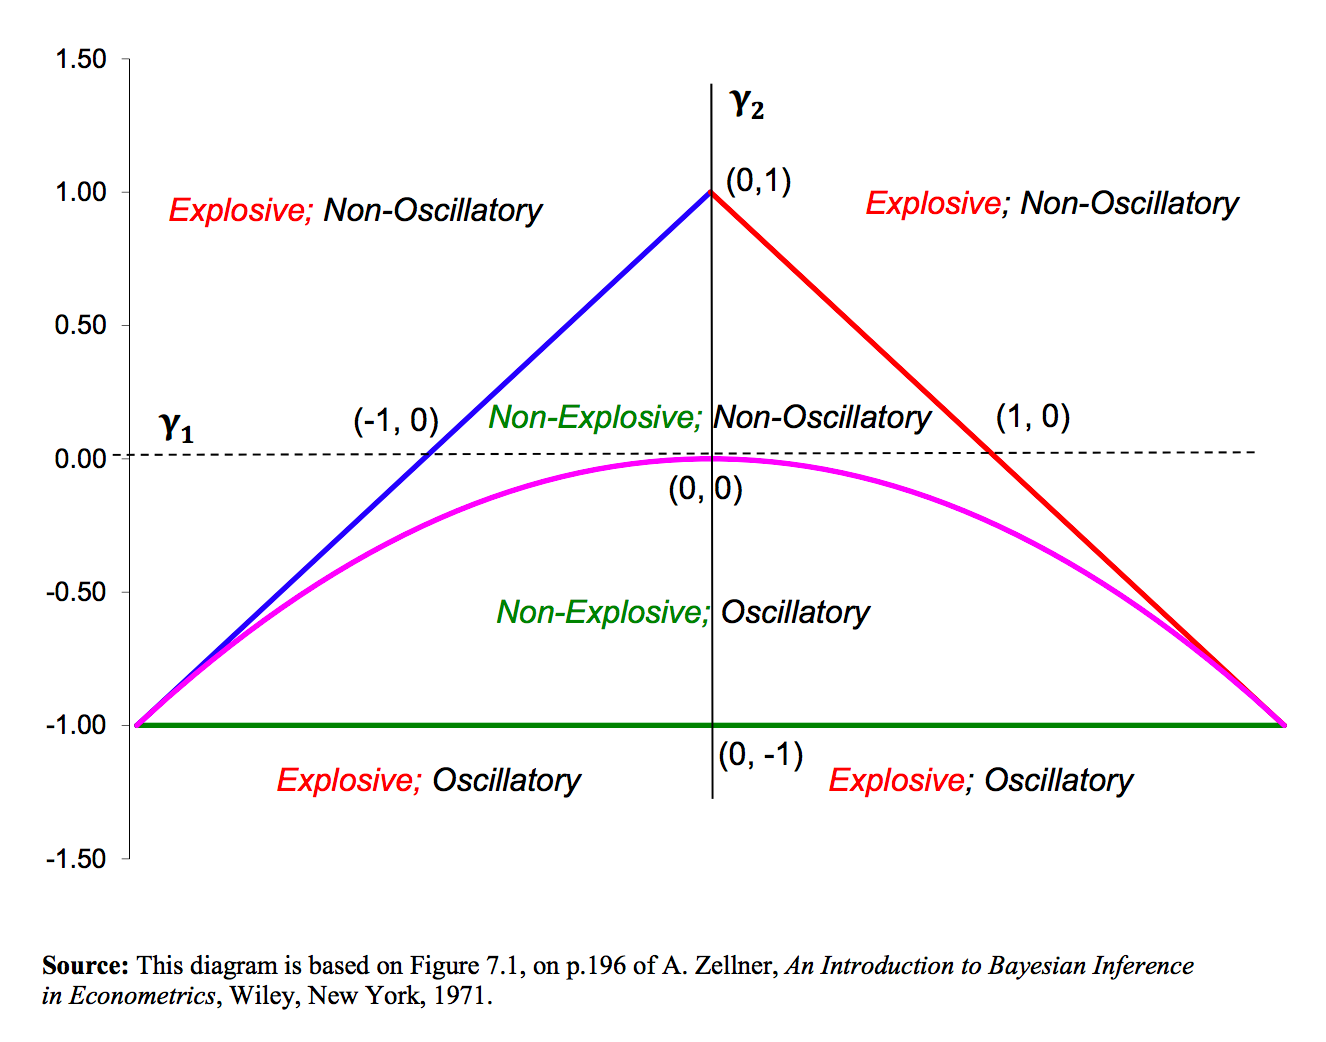
\includegraphics[width=0.85\textwidth]{figs/ar2_conditions.png}
\end{center}

\tiny{From \url{http://www.sfu.ca/~baa7/Teaching/econ818/StationarityAR2.pdf}}

\end{frame}

\begin{frame}{Proof}

We can rewrite the \(AR(p)\) model into an \(AR(1)\) form using matrix
notation

\[
\begin{aligned}
y_t &= \delta + \phi_1 \, y_{t-1} + \phi_2 \, y_{t-2} + \cdots + \phi_p \, y_{t-p} + w_t  \\
\bm\xi_t &= \bm{\delta} + \bm{F} \, \bm\xi_{t-1} + \bm w_t
\end{aligned}
\] where \[
\begin{aligned}
\begin{bmatrix}
y_t \\
y_{t-1} \\
y_{t-2} \\
\vdots \\
y_{t-p+1}
\end{bmatrix} 
&=
\begin{bmatrix}
\delta \\
0 \\
0 \\
\vdots \\
0
\end{bmatrix}
+
\begin{bmatrix}
\phi_1 & \phi_2 & \phi_3 & \cdots & \phi_{p-1} & \phi_p \\
1 & 0 & 0 & \cdots & 0 & 0 \\
0 & 1 & 0 & \cdots & 0 & 0 \\
\vdots & \vdots & \vdots & \cdots & \vdots & \vdots \\
1 & 0 & 0 & \cdots & 1 & 0 \\
\end{bmatrix} 
\begin{bmatrix}
y_{t-1} \\
y_{t-2} \\
y_{t-3} \\
\vdots \\
y_{t-p}
\end{bmatrix} 
+
\begin{bmatrix}
w_t \\
0 \\
0 \\
\vdots \\
0
\end{bmatrix} \\
&=
\begin{bmatrix}
\delta + w_t + \sum_{i=1}^p \phi_i \, y_{t-i} \\
y_{t-1} \\
y_{t-2} \\
\vdots \\
y_{t-p+1}
\end{bmatrix}
\end{aligned}
\]

\end{frame}

\begin{frame}[t]{Proof sketch (cont.)}

So just like the original \(AR(1)\) we can expand out the autoregressive
equation

\[
\begin{aligned}
\bm\xi_t 
  &= \bm{\delta} + \bm w_t + \bm{F} \, \bm\xi_{t-1}  \\
  &= \bm{\delta} + \bm w_t + \bm{F} \, (\bm\delta+\bm w_{t-1}) + \bm{F}^2 \, (\bm \delta+\bm w_{t-2}) + \cdots \\
  &\qquad\qquad~\,\,\,                        + \bm{F}^{t-1} \, (\bm \delta+\bm w_{1}) + \bm{F}^t \, (\bm \delta+\bm w_0) \\
  &= \bm{\delta} \sum_{i=0}^t F^i + \sum_{i=0}^t F^i \, w_{t-i}
\end{aligned}
\]

and therefore we need \(\underset{t\to\infty}{\lim} F^t \to 0\).

\end{frame}

\begin{frame}[t]{Proof sketch (cont.)}

We can find the eigen decomposition such that
\(\bm F = \bm Q \bm \Lambda \bm Q^{-1}\) where the columns of \(\bm Q\)
are the eigenvectors of \(\bm F\) and \(\bm \Lambda\) is a diagonal
matrix of the corresponding eigenvalues.

A useful property of the eigen decomposition is that

\[ \bm{F}^i = \bm Q \bm \Lambda^i \bm Q^{-1} \]

\pause

Using this property we can rewrite our equation from the previous slide
as

\[
\begin{aligned}
\bm\xi_t 
  &= \bm{\delta} \sum_{i=0}^t F^i + \sum_{i=0}^t F^i \, w_{t-i} \\
  &= \bm{\delta} \sum_{i=0}^t \bm Q \bm \Lambda^i \bm Q^{-1} + \sum_{i=0}^t \bm Q \bm \Lambda^i \bm Q^{-1} \, w_{t-i}
\end{aligned}
\]

\end{frame}

\begin{frame}[t]{Proof sketch (cont.)}

\[
\bm \Lambda^i = \begin{bmatrix}
\lambda_1^i & 0 & \cdots & 0 \\
0 & \lambda_2^i & \cdots & 0 \\
\vdots & \vdots & \ddots & \vdots \\
0 & 0 & \cdots & \lambda_p^i \\
\end{bmatrix}
\]

Therefore, \[\underset{t\to\infty}{\lim} F^t \to 0\] when
\[\underset{t\to\infty}{\lim} \Lambda^t \to 0\] which requires that
\[|\lambda_i| < 1 \;\; \text{ for all} \; i\]

\end{frame}

\begin{frame}{Proof sketch (cont.)}

Eigenvalues are defined such that for \(\bm \lambda\),

\[ \det (\bm{F}-\bm\lambda\,\bm{I}) = 0\]

based on our definition of \(\bm F\) our eigenvalues will therefore be
the roots of

\[\lambda^p -\phi_1\,\lambda^{p-1}-\phi_2\,\lambda^{p-2} - \cdots - \phi_{p_1} \, \lambda^1 - \phi_p = 0\]

\pause

which if we multiply by \(1/\lambda^p\) where \(L = 1/\lambda\) gives

\[1 -\phi_1\,L-\phi_2\,L^2 - \cdots - \phi_{p_1} \, L^{p-1} - \phi_p \, L^p = 0\]

\end{frame}

\begin{frame}{Properties of \(AR(p)\)}

For a \emph{stationary} \(AR(p)\) process where \(w_t\) has
\(E(w_t) = 0\) and \(Var(w_t) = \sigma_w^2\)

\[ 
\begin{aligned}
E(Y_t) &= \frac{\delta}{1-\phi_1 -\phi_2-\cdots-\phi_p} \\
\\
Var(Y_t) &= \gamma_0 = \phi_1\gamma_1 + \phi_2\gamma_2 + \cdots + \phi_p\gamma_p + \sigma_w^2 \\
\\
Cov(Y_t,Y_{t-j}) &= \gamma_j = \phi_1\gamma_{j-1} + \phi_2\gamma_{j-2} + \cdots + \phi_p\gamma_{j-p} \\
\\
Corr(Y_t,Y_{t-j}) &= \rho_j = \phi_1\rho{j-1} + \phi_2\rho{j-2} + \cdots + \phi_p\rho_{j-p}
\end{aligned}
\]

\end{frame}

\section{Moving Average (MA)
Processes}\label{moving-average-ma-processes}

\begin{frame}[t]{MA(1)}

A moving average process is similar to an AR process, except that the
autoregression is on the error term.
\[ MA(1): \qquad y_t = \delta + w_t + \theta \, w_{t-1} \]

Properties:

\end{frame}

\begin{frame}{Time series}

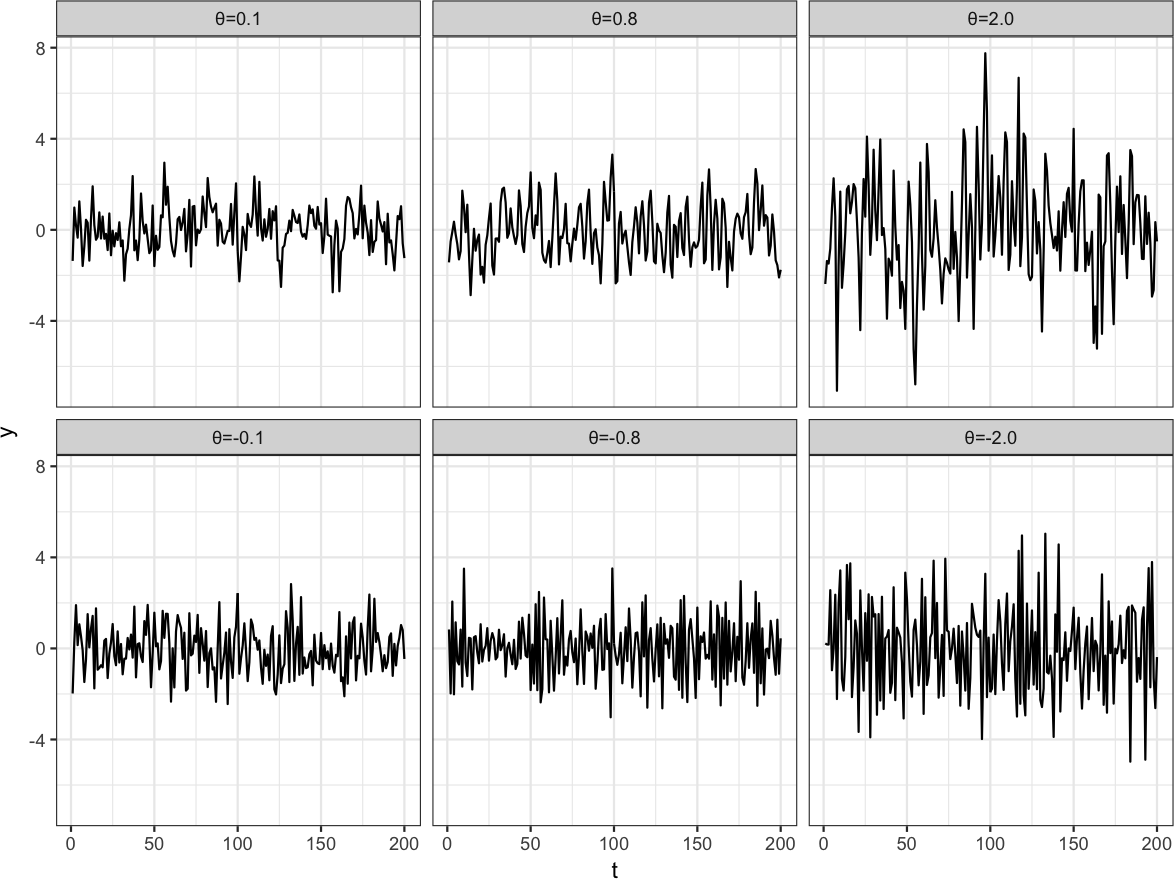
\includegraphics{Lec8_files/figure-beamer/unnamed-chunk-1-1.png}

\end{frame}

\begin{frame}{ACF}

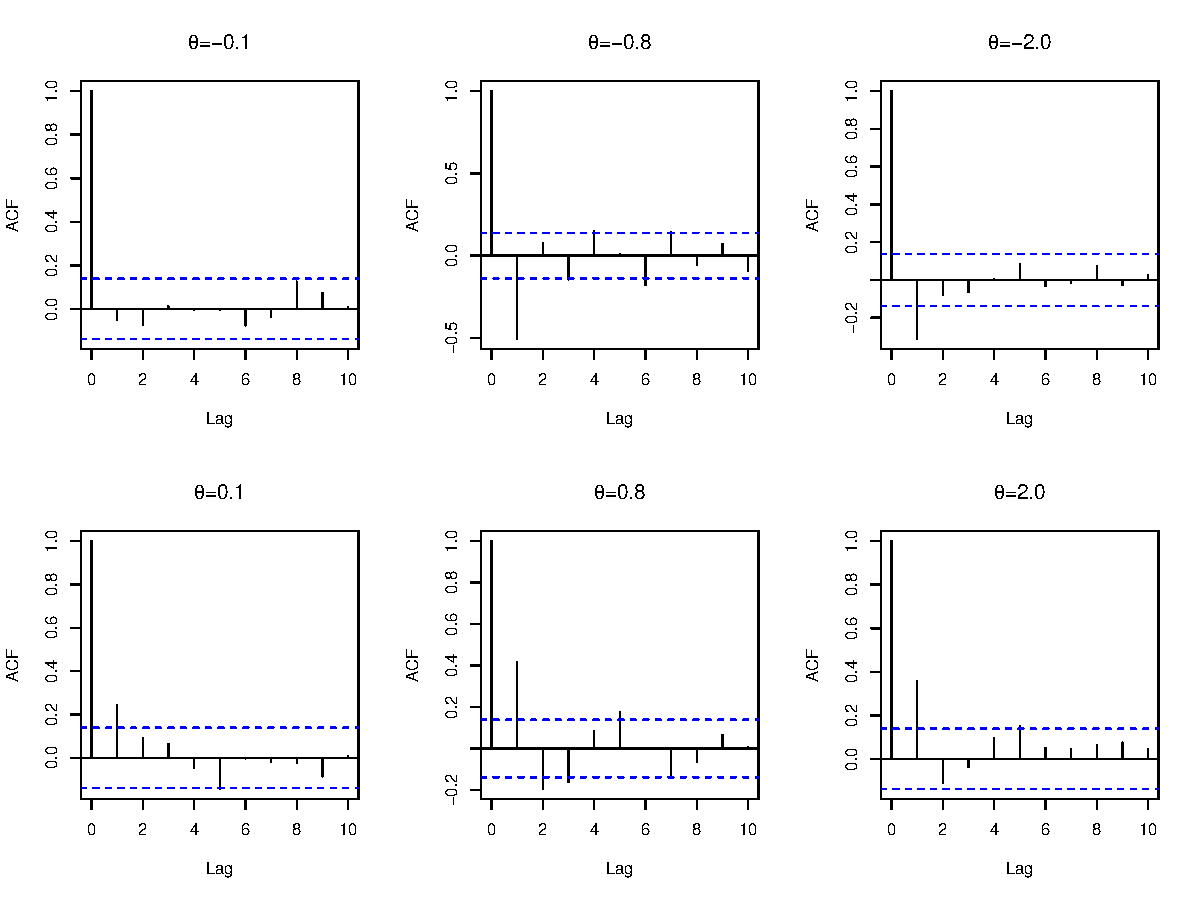
\includegraphics{Lec8_files/figure-beamer/unnamed-chunk-2-1.pdf}

\end{frame}

\begin{frame}[t]{MA(q)}

\[ MA(q): \qquad y_t = \delta + w_t + \theta_1 \, w_{t-1} + \theta_2 \, w_{t-2} + \cdots + \theta_q \, w_{t-q} \]

Properties:

\end{frame}

\begin{frame}{Time series}

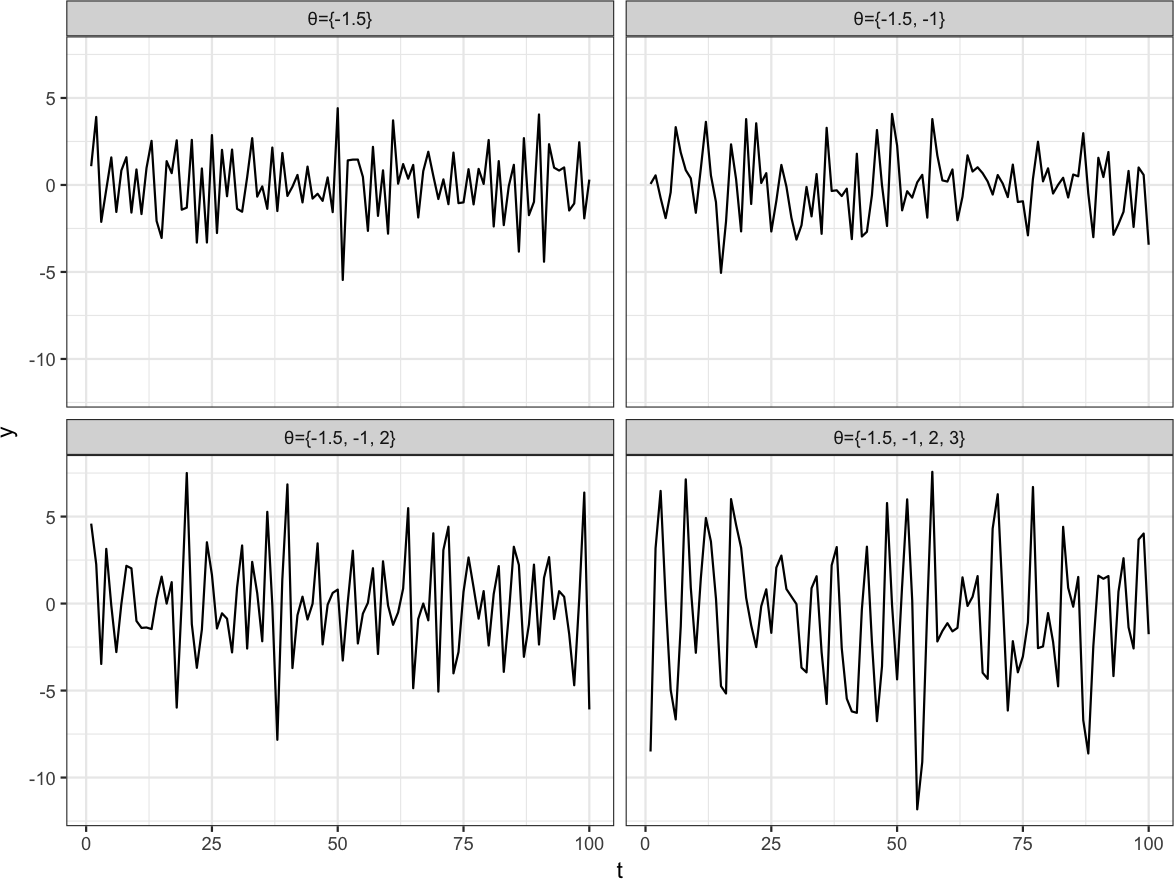
\includegraphics{Lec8_files/figure-beamer/unnamed-chunk-3-1.png}

\end{frame}

\begin{frame}{ACF}

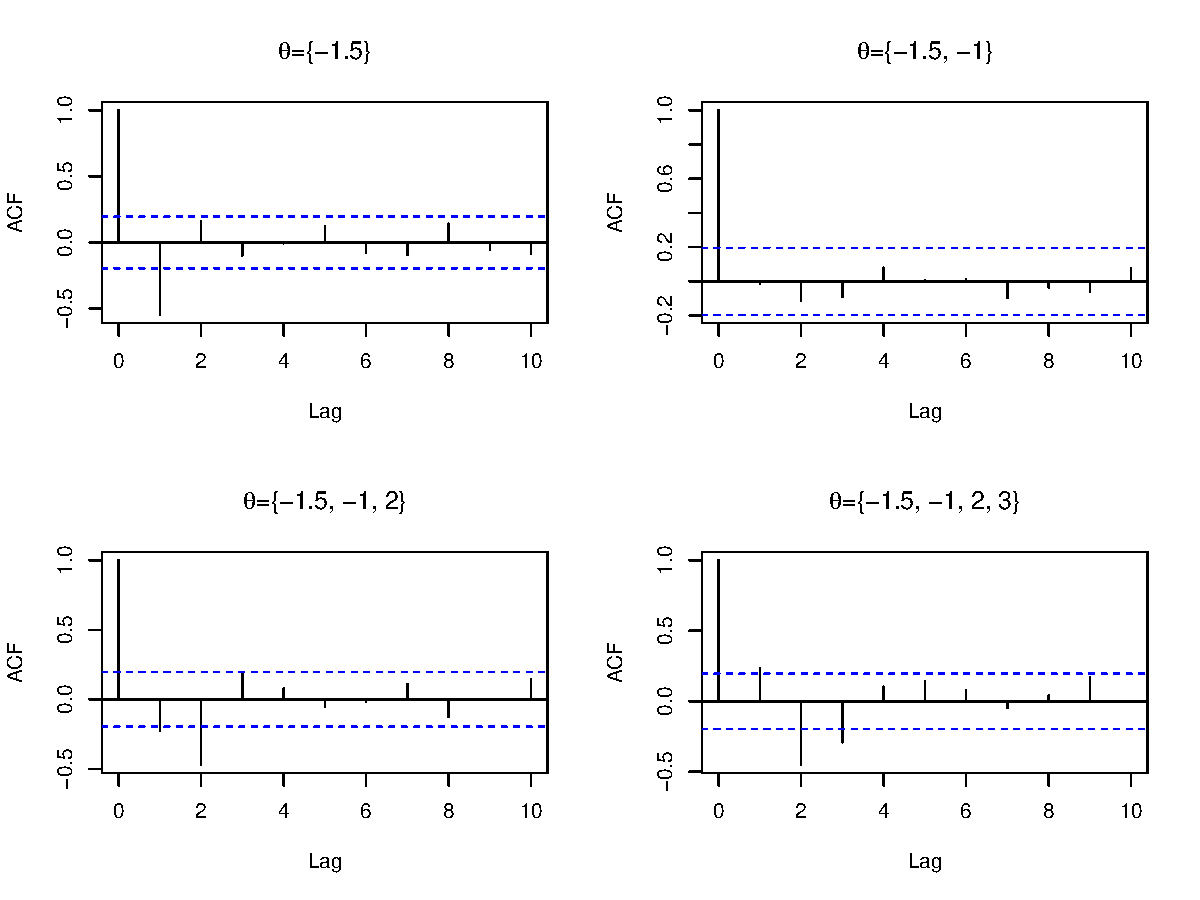
\includegraphics{Lec8_files/figure-beamer/unnamed-chunk-4-1.pdf}

\end{frame}

\section{ARMA Model}\label{arma-model}

\begin{frame}[t]{ARMA Model}

An ARMA model is a composite of AR and MA processes,

\[
\begin{aligned}
ARMA(p,q): \quad\quad\\
   y_t &= \delta + \phi_1 \, y_{t-1} + \cdots \phi_p \, y_{t-p} + w_{t} + \theta_1 w_{t-1} + \cdots + \theta_q w_{t_q} \\
  \phi_p(L) y_t &= \delta + \theta_q(L)w_t 
\end{aligned}
\]

Since all \(MA\) processes are stationary, we only need to examine the
\(AR\) aspect to determine stationarity (roots of \(\phi_p(L)\) lie
outside the complex unit circle).

\end{frame}

\begin{frame}{Time series}

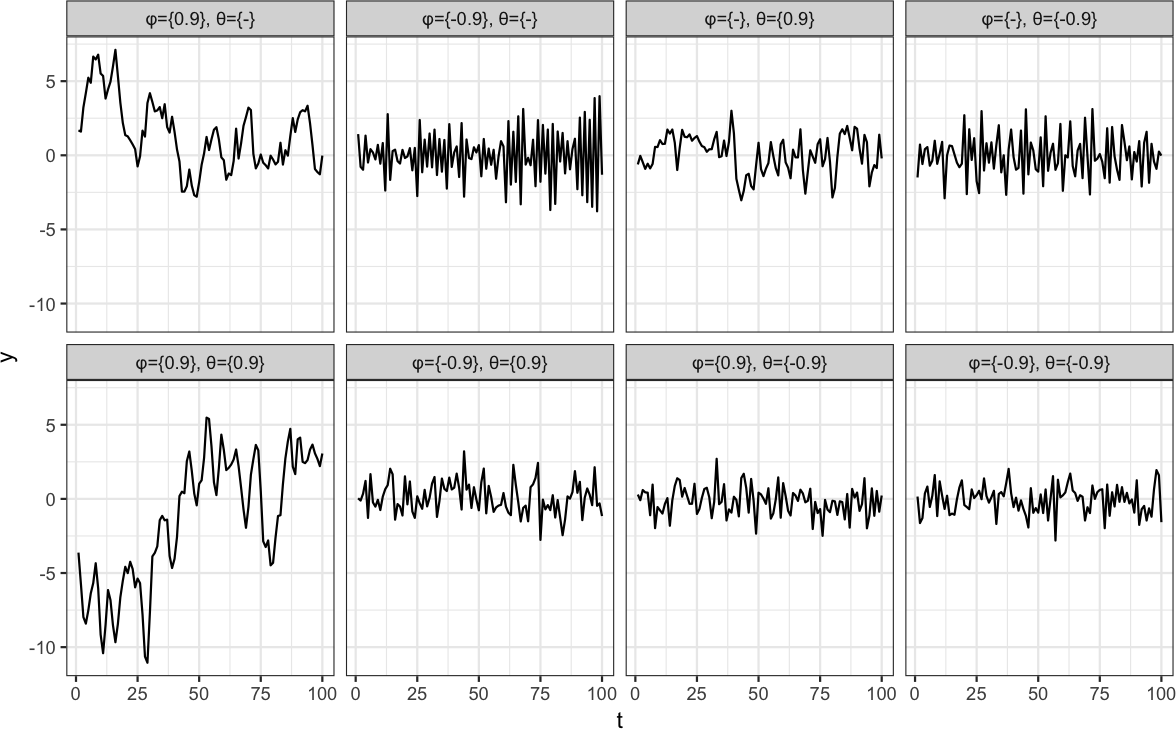
\includegraphics[width=1.2\textwidth]{Lec8_files/figure-beamer/unnamed-chunk-5-1}

\end{frame}

\begin{frame}{ACF}

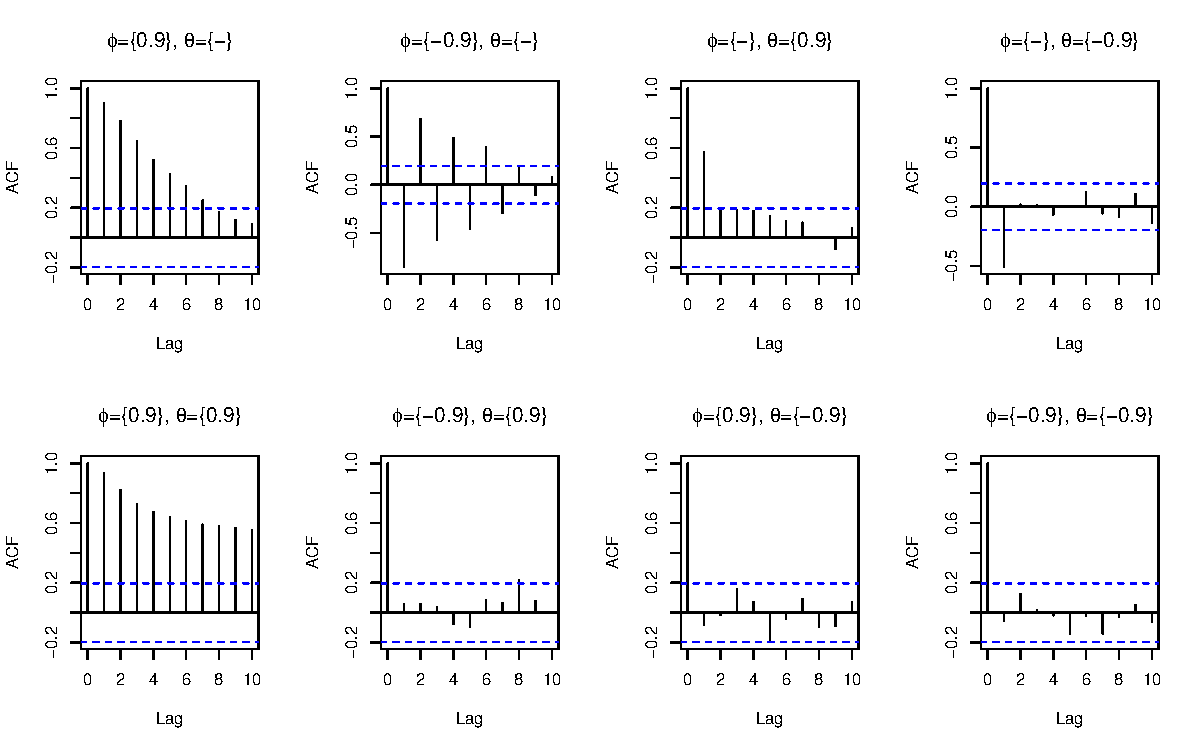
\includegraphics[width=1.2\textwidth]{Lec8_files/figure-beamer/unnamed-chunk-6-1}

\end{frame}

\end{document}
